\chapter{序論}
\label{chap:introduction}

本章では、本研究の背景と目的、及び本論文の構成について述べる。

\newpage

\section{背景}

アプリケーションランチャーはオペレーティングシステムに標準で搭載されているだけでなく、サードパーティ製としても多くのソフトウェアが開発/公開されている。ホットキー型のランチャー以外にも異なるインターフェースを持ったランチャーが数多く存在しており、それぞれ異なった利点/欠点がある。

\subsection{アプリケーションランチャーの種類と比較}

アプリケーションランチャーには以下のような種類があり、その特徴に合わせて様々な方法でアプリケーションを起動することができる。

\subsubsection{パレット型}

画面上の一部に固定されたパレット型のエリアにアプリケーションを登録し、マウスによるクリックで起動するタイプのランチャー。macOSにおけるDock(図\ref{fig:dock})がこれにあたる。デスクトップに常駐していることから簡単にアクセスでき、誰でも使いやすいものとなっている。しかしそのエリアは限られており、多くのアプリケーションを登録しようとすると、ボタン数を増やしたりそれぞれを小さく表示したりする必要がある。基本的にその数が増えれば増えるほど操作性が低下するため、数個から数十個の頻用するアプリケーションを登録して使用するのが推奨される。

\begin{figure}[h]
    \begin{center}
       \fbox{
\includegraphics[width=100mm]{images/dock}}
    \end{center}
    \caption{Dock}
    \label{fig:dock}
\end{figure}

\subsubsection{メニュー型}

上述したDock等にメニューを設け、マウスを使用して登録したアプリケーションを起動できるようにするタイプのランチャー。ショートカットキーと組み合わせて使用されるものもある。複数のアプリケーションを一つにまとめることで場所を節約できるだけでなく、階層化によって自分の使いやすいように整理することもできる。しかし、項目や階層が増えれば目的のアプリケーションに辿り着くまでの操作ステップは増えることになる。

\newpage

\begin{figure}[h]
    \begin{center}
       \fbox{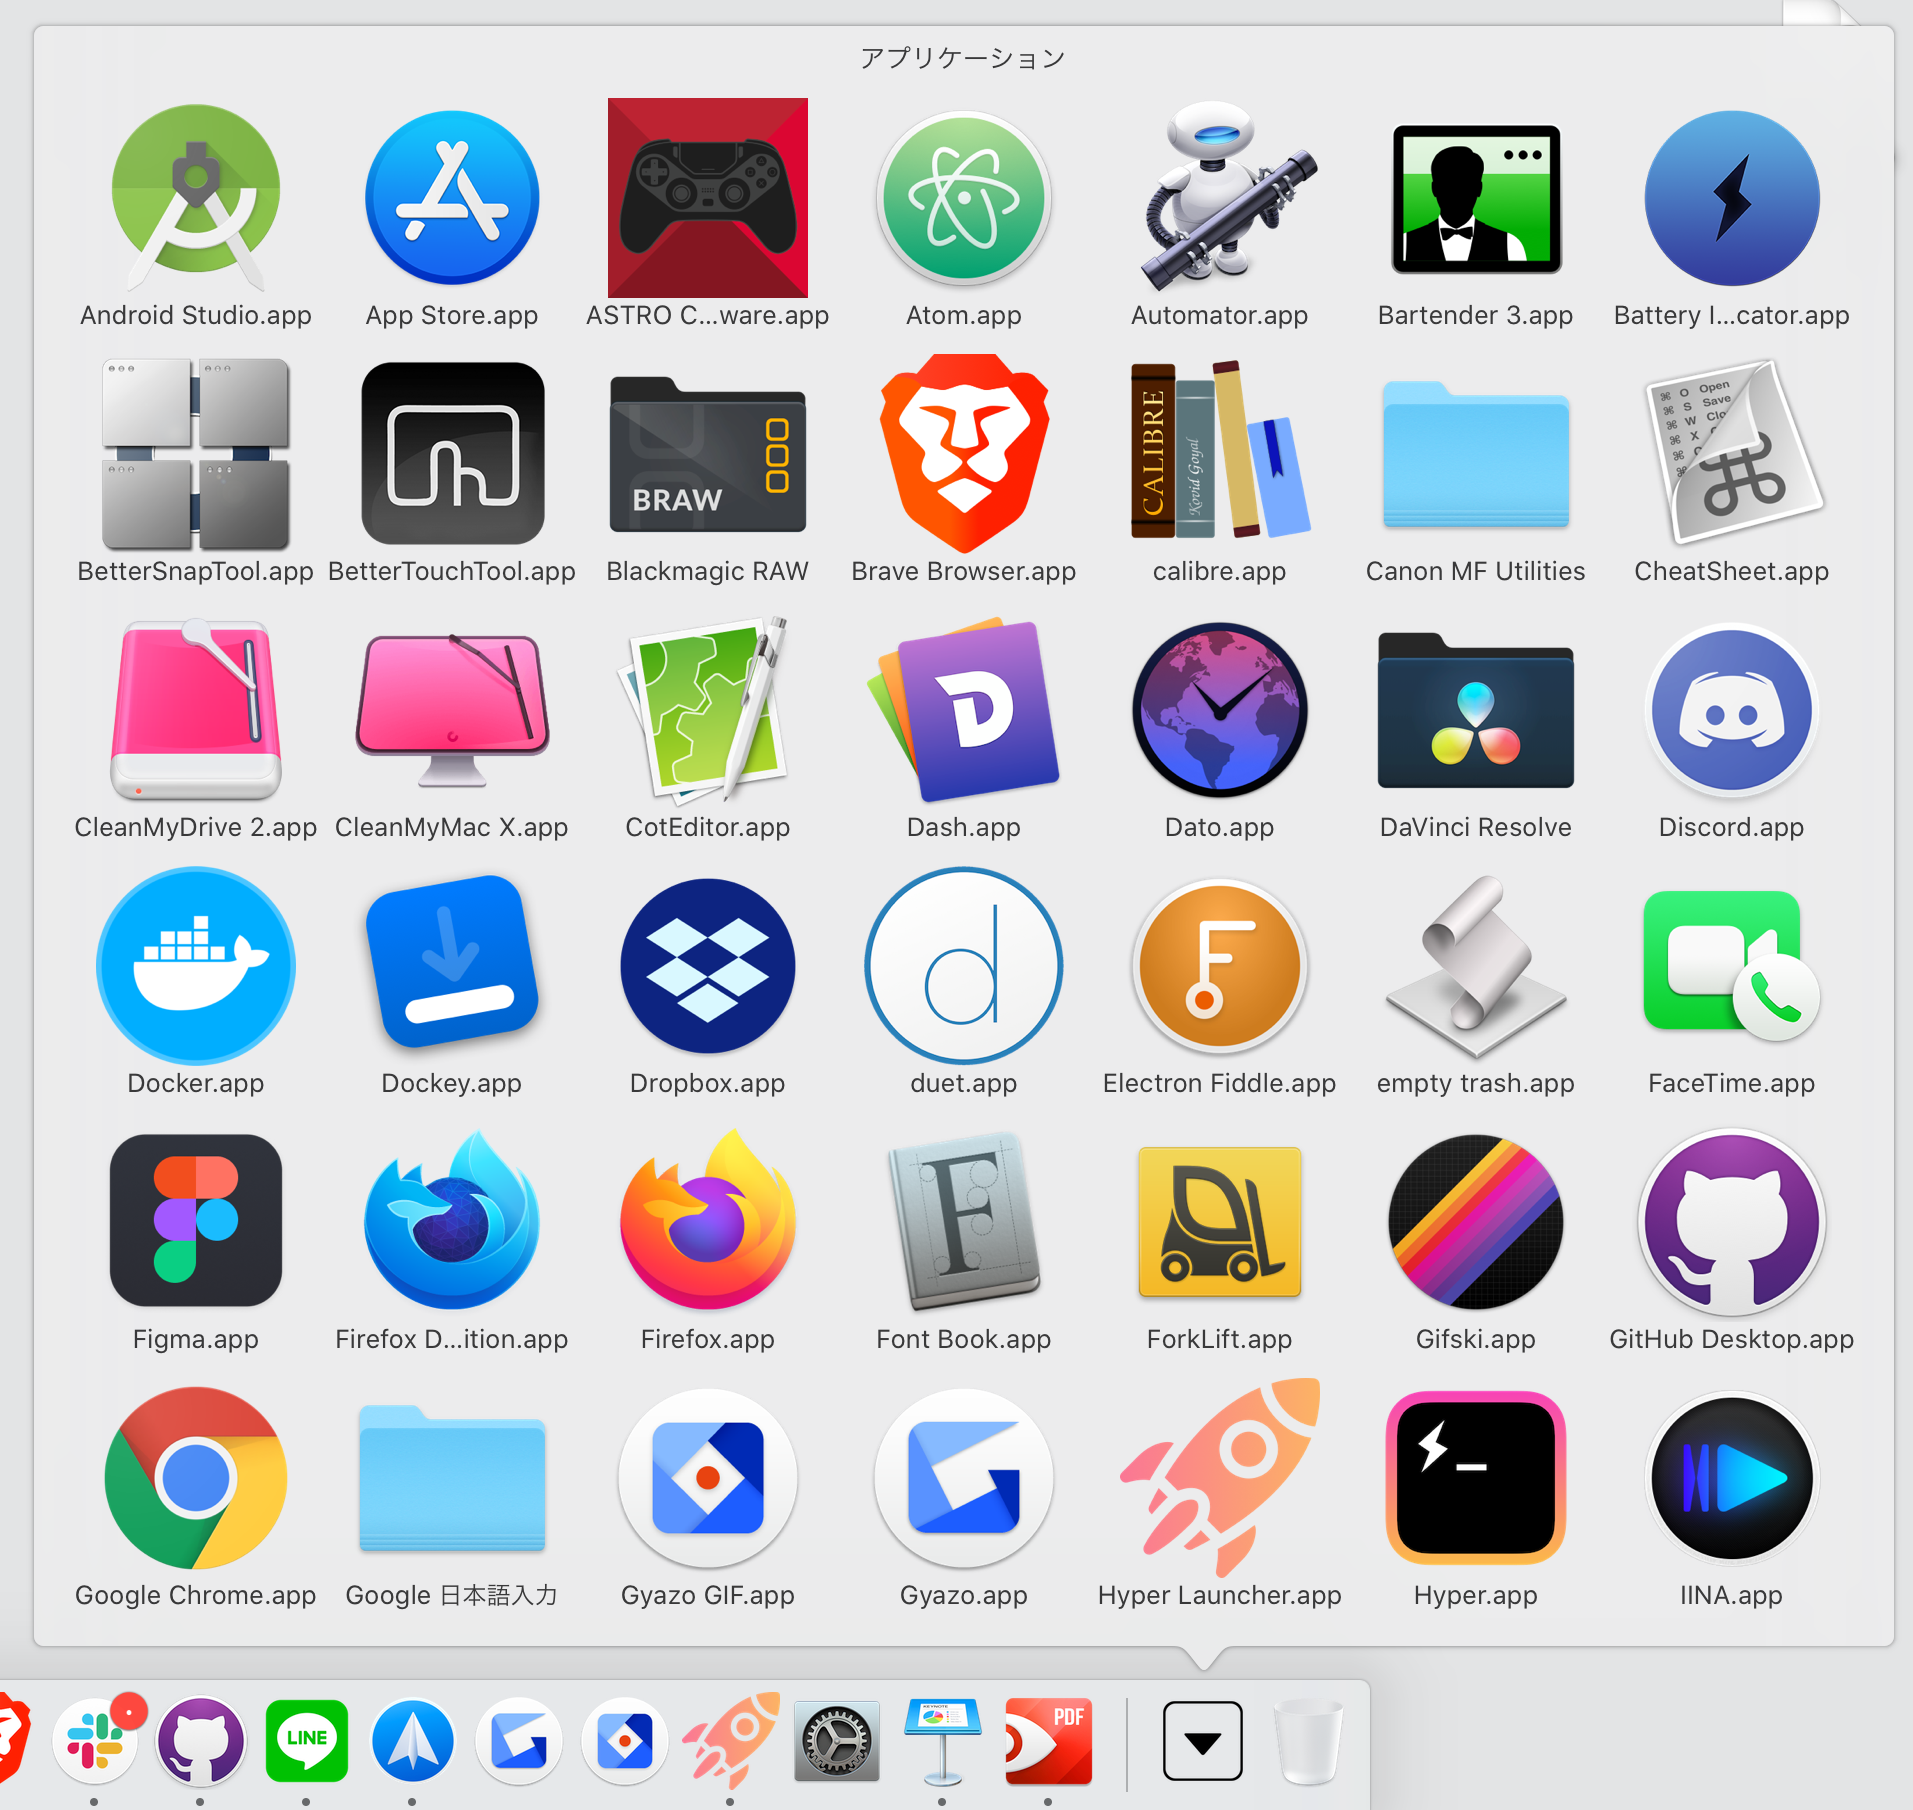
\includegraphics[width=100mm]{images/menu}}
    \end{center}
    \caption{Dock内のメニュー}
    \label{fig:menu}
\end{figure}

\subsubsection{検索型}

アプリケーションの名前を入力することで対象のアプリケーションを検索し起動するタイプのランチャー。macOSにおけるSpotlightがこれにあたる。検索メニューは使用するときのみ表示されるため使用していない時は場所をとらず、キーボードのみの操作で完結しているのも利点の一つである。もちろんマウスと組み合わせて使用することもできる。また大抵の場合インクリメンタルサーチが導入されているため、名前を全て覚えていなくても起動することができる。しかし汎用性が高い反面、毎回一定のキーボード入力が必要となってしまうというのが欠点である。

\begin{figure}[h]
    \begin{center}
       \fbox{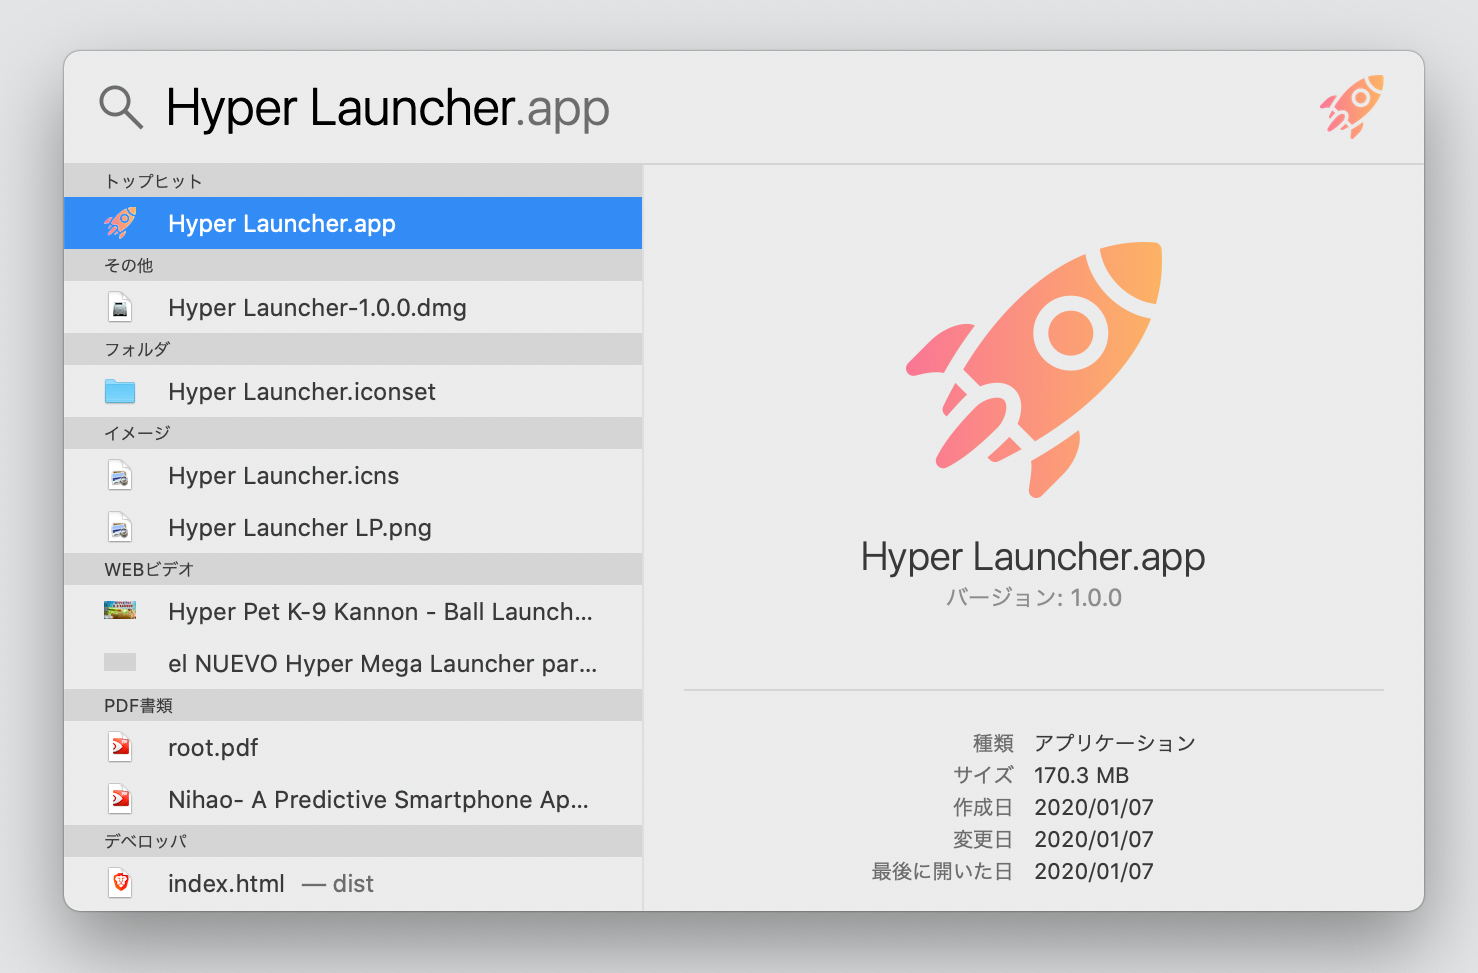
\includegraphics[width=100mm]{images/spotlight}}
    \end{center}
    \caption{Spotlight}
    \label{fig:spotlight}
\end{figure}

\subsubsection{ホットキー型}

単一のキーもしくは複数のキーの組み合わせを入力するだけで、登録したアプリケーションを起動できるタイプのランチャー。今回着目しているのがこのである。他のとは違い、ホットキー型は標準で搭載されていないことがほとんどである。したがって自分に適したサードパーティ製ソフトウェアを探してくる必要がある。画面上に情報を表示する必要がなく場所を取らないことに加え、一発で特定のアプリケーションを起動できるため、とても強力なランチャーである。しかし設定が面倒であったり、どのキーにどのアプリケーションを登録したのか覚えておく必要があったりと、初心者には使いにくいタイプだとされているのも事実である。これこそが標準として機能が提供されていない理由の一つだと考えられる。

\subsection{既存のアプリケーションの問題点}

先述した通り、ホットキーを利用したアプリケーションランチャーは標準で搭載されておらず、使用者自ら使いやすいものを探す必要がある。しかしその種類は豊富とは言えず、突出した特徴があるわけでもない。例として筆者が日常的に使用してきた2つのアプリケーションランチャーを示す

\subsubsection{PMenu}

PMenu\footnote{https://danadesign.ltd/}(図\ref{fig:pmenu})はホットキーとメニューを利用したランチャーで、アプリケーションだけでなく様々なファイルをコマンドで操作することができる。使い勝手はいたって普通で可もなく不可もなしと言ったところである。自分の好きなホットキーを割り当てられるのは便利であるが、キーを登録するためのステップが多くとても煩雑である。コンテキストメニューを利用することが主な方法とされているため、ホットキーに関しては最低限の機能が実装されているだけと言える。

\begin{figure}[h]
    \begin{center}
       \fbox{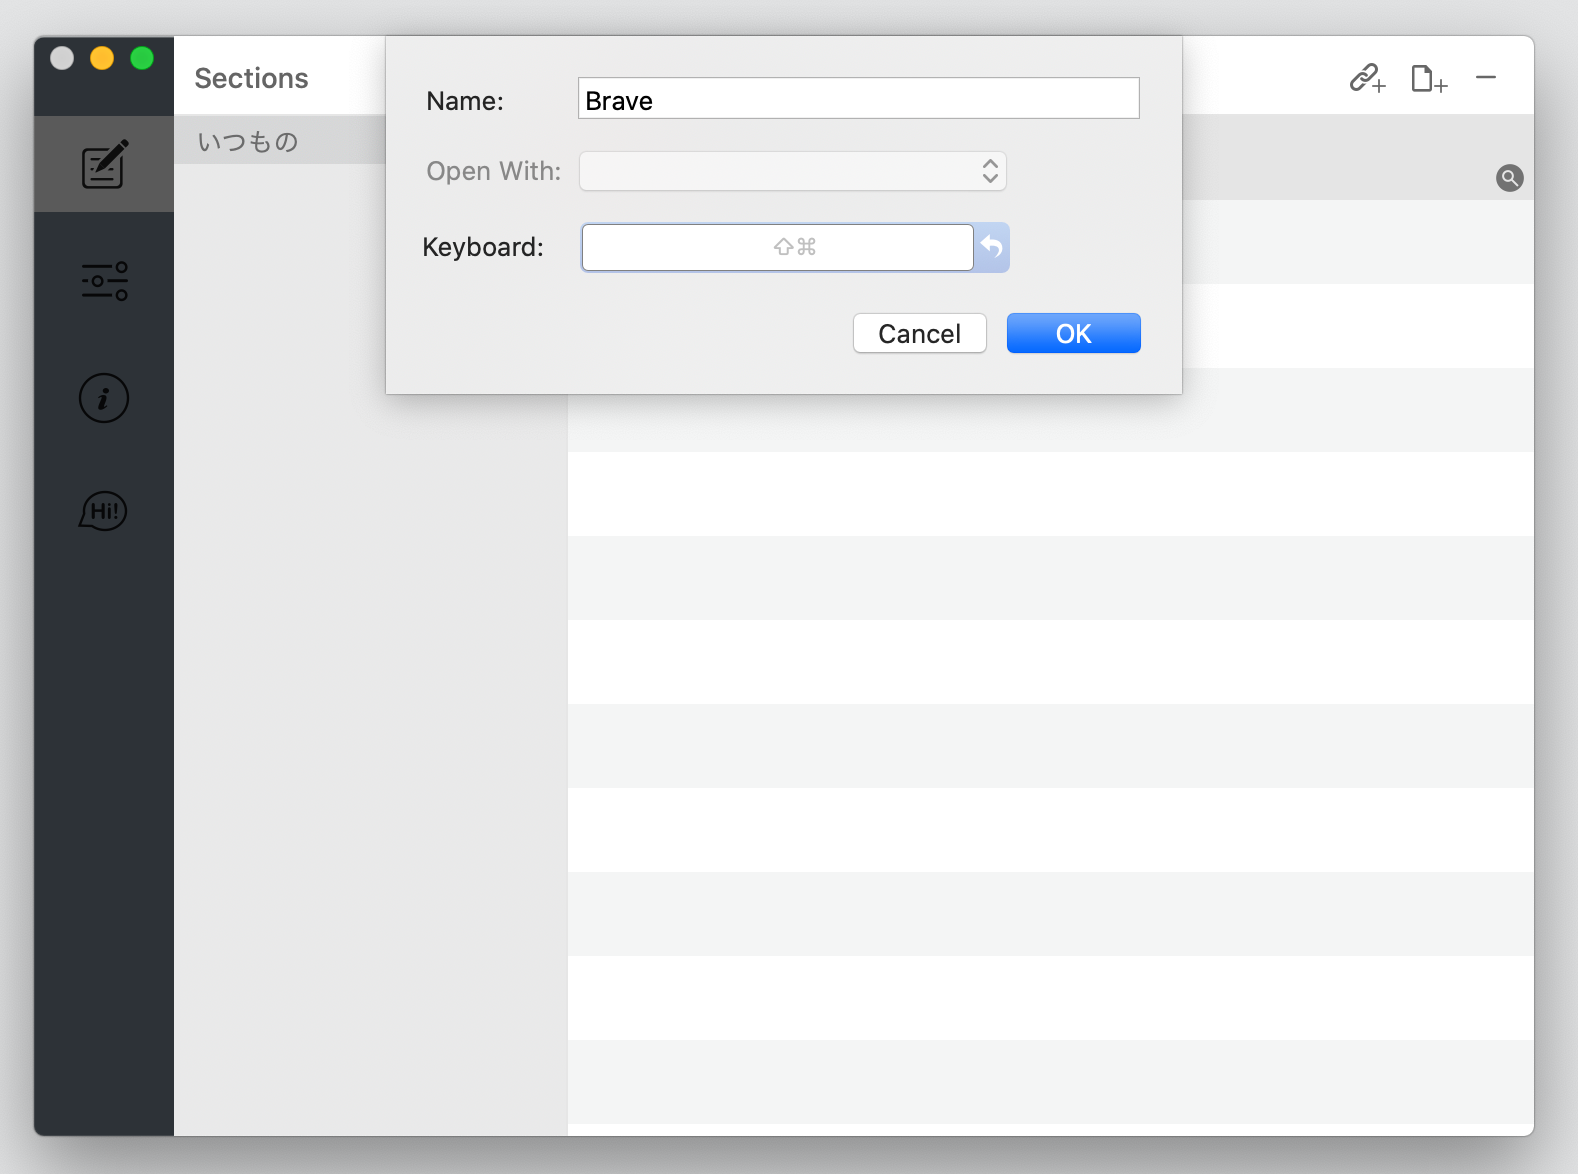
\includegraphics[width=100mm]{images/pmenu}}
    \end{center}
    \caption{PMenu}
    \label{fig:pmenu}
\end{figure}

\subsubsection{Snap}

Snap\footnote{https://apps.apple.com/jp/app/snap/id418073146}(図\ref{fig:snap})はホットキーを利用したランチャーで、macOSのDockを生かした機能が備わっている。SnapではDockに登録されたアプリケーションに左から順に数字を割り当てていき、その数字と設定したモディファイアキーとの組み合わせでアプリケーションを起動できるようになっている。これにより面倒な設定をすることなくホットキーの恩恵を授かることが可能となる。ただしDockのサイズは有限であり画面上に場所もとるため、多くのアプリケーションを登録するというのはあまり現実的ではない。

\begin{figure}[h]
    \begin{center}
       \fbox{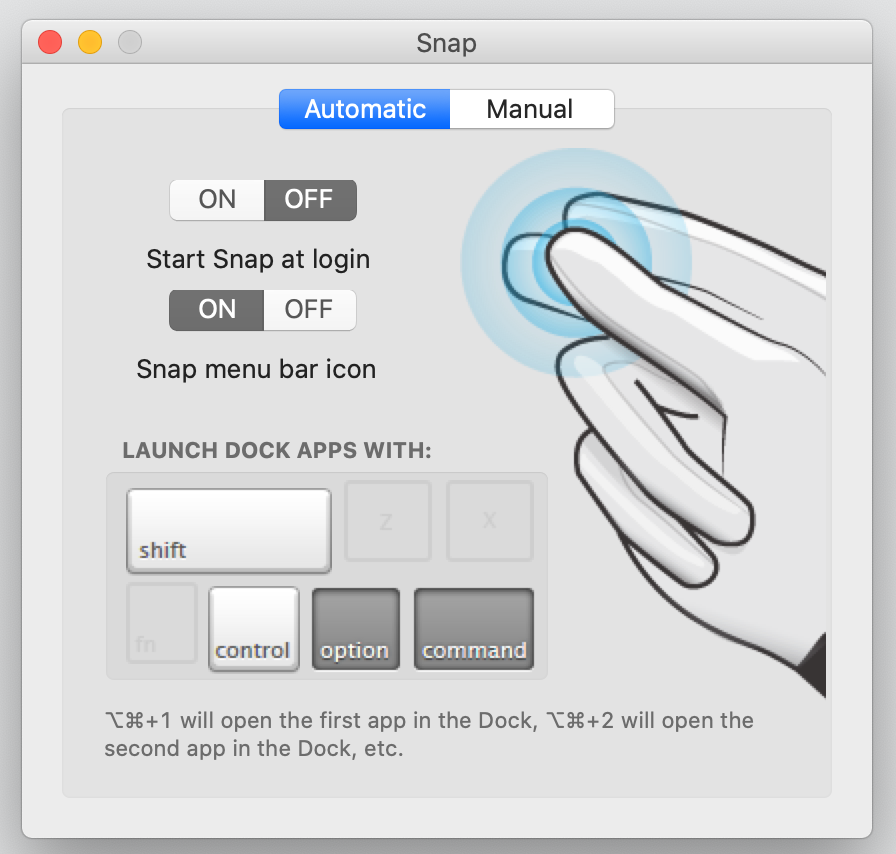
\includegraphics[width=100mm]{images/snap}}
    \end{center}
    \caption{Snap}
    \label{fig:snap}
\end{figure}

\section{本研究の目的}

既存のホットキーを利用したアプリケーションランチャーにおける不便を解消し、より強力でより多くの人に使いやすいシステムを開発することが本研究の目的である。

\section{本論文の構成}

第1章では、本研究における背景と問題意識、目的について述べた。第2章では、第1章で述べた問題意識を踏まえ、新しいホットキー型アプリケーションランチャーシステムを提案する。第3章ではシステムの実装に関して述べ、第4章では関連研究について述べる。第5章ではシステムの考察を行い、第6で本研究を総括する。